\documentclass[a4paper]{article}

\usepackage{fullpage} % Package to use full page
\usepackage{parskip} % Package to tweak paragraph skipping
\usepackage{tikz} % Package for drawing
\usepackage{amsmath}
\usepackage{amssymb}
\usepackage{hyperref}
\usepackage{multirow}
\usepackage{booktabs}


\title{Programming Assignment 1 : Minimum Spanning Trees}
\author{HUIDS: 90978217 AND MELLY'S HUID}
\date{02/27/2017}

\begin{document}

\maketitle

\section{Overview}
In this programming assignment, we constructed minimum spanning trees (MSTs) for complete undirected graphs of 0, 2, and 4 dimensions. We then determined how the average total weight of the MST grew as a function of the number of vertices $n$.

We implemented Prim's algorithm to build MSTs for graphs of each dimension for various values of $n$. Then, we plotted how the average total MST weight grew as a function of $n$. The results from our studies are presented in this report.


\section{Methods}
\subsection{Algorithm}
We chose to implement the eager implementation of Prim's algorithm. Unlike the lazy implementation of Prim's algorithm, which keeps track of all the edges connecting the MST to any vertex not in the MST, the eager implementation only keeps track of the \textbf{minimum} edges connecting each vertex not in the tree to a vertex in the tree. This way, the number of edges we need to keep track of is $O(V)$, not $O(E)$ as in the Prim's lazy implementation.

Likewise, Kruskal's algorithm also requires $O(E)$ space, because we must keep track of all edges not in the MST. Therefore, because the eager implementation of Prim's algorithm takes only $O(V) = O(n)$ space, as opposed to Kruskal's which takes $O(E) = O(n^2)$ space, we decided to implement Prim's.

\subsection{Implementation}
Our eager implementation of Prim's algorithm uses two main classes:

\begin{itemize}
	\item \texttt{Vertex}: Represents a vertex in the complete graph. The main attributes are:
	\begin{itemize}
		\item \texttt{minimum-distance}: Minimum distance (edge weight) connecting this vertex to the current MST. Whenever a new vertex $v$ is added to the MST, each edge leaving $v$ is ``relaxed''; the \texttt{minimum-distance} of neighbor $u$ is updated only if the weight of edge$(v, u_i)$ is smaller than the current minimum distance. This value fixes once a vertex is added to the MST, and allows us to calculate the final weight of the MST.
		\item \texttt{coordinates}: An array holding the vertex's coordinates, if applicable. Allows us to calculate the edge weights for Euclidean graphs.
		\item \texttt{key}: Unique integer key between 0 (inclusive) and the number of points (exclusive) associated with each vertex. Allows us to reference vertices in the priority queue.
	\end{itemize}
	Note that \texttt{Vertex} does not keep an adjacency list in memory. Because we are only generating MST's on complete graphs, where all possible edges between $n$ points exist, we can simply iterate through all entries in the current priority queue (which is initialized to all vertices) to touch all neighbors of a vertex not already in the MST. This is correct because we always maintain the invariant that the priority queue contains only those vertices not already in the MST. 
	
	\item \texttt{RandMST}: Represents a MST on a complete graph. The main attributes are: 
	\begin{itemize}
		\item \texttt{graph}: An array holding all $n$ vertices in the graph, where the vertex with key $i$ is in position $i$.
		\item \texttt{priority-queue}: A binary heap implementation of the priority queue; the queue is an integer array containing vertex keys, where the first element is the top of the heap. We use a integer variable to track the ``end'' of the queue, and never modify the size of the array.
	\end{itemize}
\end{itemize}

Additionally, we make use of a general \texttt{Experiment} object, which is passed into the constructor for Random MST's. The experiment object has methods for calculating the weight of any given edge, and for creating a new graph with random vertices, allowing us to generalize our code for many types of random spanning trees. By storing only those edges found in the final MST, our implementation of Prim's algorithm uses $O(V)$ space. Additionally, note that all edges are relaxed exactly once (potentially calling an ``increase key'' operation each time) and a minimum is extracted from the heap $V$ times. Thus, the total running time of our algorithm is bounded by $O(E\log V) = O(n^2\log n)$.

\section{Results and Discussion}
After running our algorithm on MSTs with vertices $n=2^7, 2^8, ..., 2^{17}$, we obtained the following results, where the output is the average MST weight:

\begin{table}[htbp]
  \centering
    \begin{tabular}{cr|rrrr}
          & \multicolumn{1}{r}{} & \multicolumn{4}{c}{\textbf{Dimension}} \\
          &       & \textbf{0} & \textbf{2} & \textbf{3} & \textbf{4} \\
\cmidrule{2-6}    \multirow{11}[1]{*}{\textbf{$\log_2n$}} & \textbf{7} & 1.113 & 7.716 & 17.833 & 28.518 \\
          & \textbf{8} & 1.181 & 10.797 & 27.597 & 46.919 \\
          & \textbf{9} & 1.188 & 14.852 & 43.057 & 78.282 \\
          & \textbf{10} & 1.190 & 21.093 & 67.795 & 130.567 \\
          & \textbf{11} & 1.197 & 29.657 & 107.295 & 216.398 \\
          & \textbf{12} & 1.200 & 41.828 & 169.348 & 360.653 \\
          & \textbf{13} & 1.201 & 58.878 & 266.873 & 603.351 \\
          & \textbf{14} & 1.201 & 83.074 & 422.195 & 1009.779 \\
          & \textbf{15} & 1.201 & 117.552 & 668.605 & 1686.334 \\
          & \textbf{16} & 1.204 & 166.121 & 1058.731 & 2827.767 \\
          & \textbf{17} & 1.202 & 234.581 & 1677.107 & 4740.367 \\
    \end{tabular}%
  \caption{Average MST weights for different values of $\log_2n$ and dimension.}
  \label{tab:addlabel}%
\end{table}%

Plotting our results in R and fitting our models using non-linear least squares analysis gives us the following graphs:

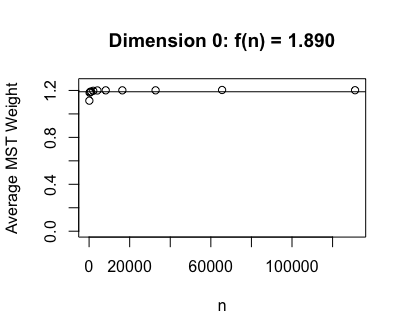
\includegraphics[width=3.4in]{dim0plot}
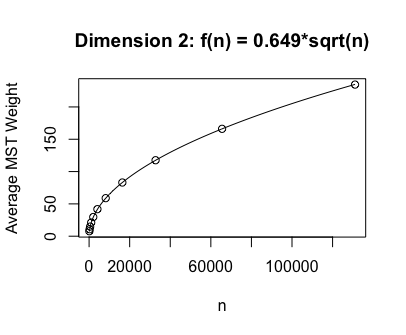
\includegraphics[width=3.4in]{dim2plot}\\
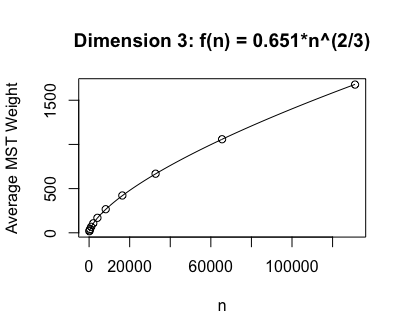
\includegraphics[width=3.4in]{dim3plot}
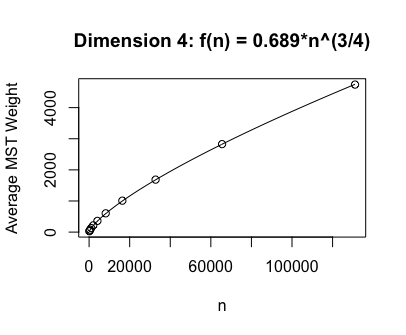
\includegraphics[width=3.4in]{dim4plot}

Based off these best fit lines, we guessed the following formula for $f(n)$ other than than dimension 0, where $d$ is the dimension:
$$f(n) = 0.65n^{\frac{d-1}{d}}$$

This growth rate is not surprising. First, we note that this function's second derivative is negative, indicating that greater values of $n$ correspond to a lesser increase in $f(n)$. This makes sense, because increasing the number of vertices while limiting the coordinates of each vertex results in vertices that are clustered more closely together, decreasing the impact of any additional vertices on total MST weight. Thus, a increase in $n$ will not result in an equally proportional increase in $f(n)$, since new vertices are likely to be closer together to existing vertices.

Second, we also note that as the numbers of dimensions increases, the growth rate of $f(n)$ approaches $O(n)$. Again, this makes sense, because increasing the number of dimensions that each vertex has access to decreases the aforementioned clustering effect; that is, adding additional vertices are less likely to result in a graph that is tightly clustered, since these extra vertices are more likely to "farther" away from existing vertices.

For the dimension 0 case, we simply modeled the relationship with a constant, because we noted that values of $f(n)$ appeared to converge to a value of around 1.2 as n increased. Intuitively, this is not surprising, because increasing $n$ here simply adds vertices to a cluster of extremely closely-connected nodes, such that adding additional vertices will not impact the minimum spanning tree distance (since any additional vertices will exist within this dense cluster).



\end{document}